% coding:utf-8

%----------------------------------------
%FOSAPHY, a LaTeX-Code for a summary of basic physics
%Copyright (C) 2013, Daniel Winz, Ervin Mazlagic

%This program is free software; you can redistribute it and/or
%modify it under the terms of the GNU General Public License
%as published by the Free Software Foundation; either version 2
%of the License, or (at your option) any later version.

%This program is distributed in the hope that it will be useful,
%but WITHOUT ANY WARRANTY; without even the implied warranty of
%MERCHANTABILITY or FITNESS FOR A PARTICULAR PURPOSE.  See the
%GNU General Public License for more details.
%----------------------------------------

\section{Einfache harmonische Schwingung}
Die einfache harmonische Schwingung beschreibt ein System, welches 
nur zwei Energiespeicher hat. Ein klassisches Beispiel
ist die an einer Feder befestigte Masse. Um ein 
schwingfähiges System zu erhalten, muss es Wirkungen geben welche
entgegengesetzt sind. Im Beispiel aus Abbildung 
\ref{fig:einfache-harmonische} gibt es die zwei Kräfte $\vec{F}_k$ und
$\vec{F}_m$ die entgegengesetzt sind.

\begin{figure}[h!]
	\centering
	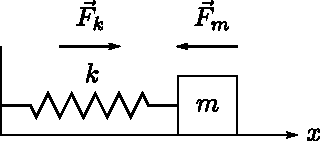
\includegraphics[scale=0.75]{../fig/einfache-harmonische.pdf}
	\caption{Einfach harmonisches Schwinungssystem}
	\label{fig:einfache-harmonische}
\end{figure}

\begin{figure}[h!]
	\centering
	\begin{tikzpicture}[domain=0:4]
		\draw[->] (-0.1,0) -- (5,0) node[below] {$t$};
		\draw[->] (0,-2.5) -- (0,2.5) node[left] {$x$};

		\draw[color=red, samples=200] plot[id=x] 
			function{0.5*cos(2*x)};
		\draw[color=blue, samples=200] plot[id=v] 
			function{-2*0.5*sin(2*x)};
		\draw[color=green, samples=200] plot[id=a] 
			function{-2*2*0.5*cos(2*x)};

		\draw[red] (4,2) node[right] 
			{$x(t) = A \sin(\omega t + \varphi)$};
		\draw[blue] (4,1.5) node[right] 
			{$\dot{x}(t) = -\omega A \cos(\omega t + \varphi)$};
		\draw[green] (4,1) node[right]
			{$\ddot{x}(t) = -\omega^2 A \sin(\omega t + \varphi)$};

		\draw[] (0.1,0.5) -- (-0.1,0.5) node[left] {$A$};
		\draw[] (0.1,1) -- (-0.1,1) node[left] {$\omega A$};
		\draw[]	(0.1,2) -- (-0.1,2) node[left] {$\omega^2 A$};
	\end{tikzpicture}
	\caption{Plot der einfachen harmonischen Schwingung}
\end{figure}

\subsection{Differentialgleichung}
Der Zusammenhang aus Abbildung \ref{fig:einfache-harmonische} stellt 
direkt die allgemeine Form des Systems als Differentialgleichung auf zu
\[ \boxed{\vec{F}_\Sigma  
	= \vec{F}_m + \vec{F}_k
	= m \cdot \ddot{x} + k \cdot x
	= 0
} \]

Der Weg, die Geschwindigkeit und die Beschleunigung lassen sich analog
zur linearen Bewegung durch Ableitungen und Integrale voneinander herleiten.
\[ \boxed{ \begin{array}{c c l}
	x(t) & = & 
		A \cdot \cos(\omega \cdot t + \varphi) \\
	\dot{x}(t) & = & 
		-\omega A \cdot \sin(\omega \cdot t + \varphi) \\
	\ddot{x}(t) & = & 
		-\omega^2 A \cdot \cos(\omega \cdot t + \varphi)
\end{array}}\]

Die Amplitude $A$ und die Phasenverschiebung $\varphi$ bietet die  
Parametierung der Bewegung an. Diese sind bei der einfachen harmonischen 
und ungedämpften Schwingung stets konstant. Die Kreisfrequenz $\omega$ 
beschreibt die Dynamik des Systems, also die \textit{Schnelligkeit}.
Diese kann aber auch mittels der Frequenz $f$ oder der Periodendauer $T$
ausgedrückt werden. 
\[ \boxed{ 
	\omega = 2 \pi f = 2 \pi \frac{1}{T}
	\quad \Rightarrow \quad
	f = \frac{\omega}{2 \pi} 
	\quad \Rightarrow \quad 
	T = \frac{2 \pi}{\omega} = \frac{1}{f} \\
} \]
Bei einfachen harmonischen Systemen wie in Abbildung 
\ref{fig:einfache-harmonische} ist die Dynamik definiert durch das
Verhältnis von Feder und Masse.
\[ \boxed{
	\omega = \sqrt{\frac{k}{m}}
}\]

\subsection{Auslenkung und Geschwindigkeit als Anfangsbedingungen}
Wird die Feder vor dem Loslassen um die Strecke $x_0$ gedehnt, gibt 
dies die Amplitude $A$ vor. 
\[ \boxed{A = \sqrt{{x_0}^2 + \left(\frac{v_0}{\omega}\right)^2}} \]
\[ \boxed{x_0 = x(0) = A \cdot \cos(\varphi)} \]
Wird die Masse nicht einfach losgelassen
sondern mit einer Geschwindigkeit $\vec{v}_0$ bewegt, dann gibt dies
die Phasenverschiebung $\varphi$ vor.
\[ \boxed{v_0 = \dot{x}(0) = - \omega \cdot A \cdot \sin(\varphi)} \]
\[ \boxed{\phi = \tan^{-1}\left(-\frac{v_0}{\omega \cdot x_0}\right)} \]
\textbf{Achtung!} Lösung kann im falschen Quadranten liegen. 
Evtl. mit $\pi$ addieren. 


\subsection{Geschwindigkeit und Beschleunigung aus Amplitude und Position}
\[ \boxed{v(t) = \sqrt{\frac{k}{m}} \cdot \sqrt{A^2 - x^2(t)}
	= \omega \sqrt{A^2 - x^2(t)}} \]
\[ \boxed{a(t) = - \frac{k}{m} \cdot x(t) = - \omega^2 x(t)} \]

\subsection{Maximale Geschwindigkeit und Beschleunigung}
\[ \boxed{v_{max} = \omega \cdot A} \]
\[ \boxed{v_{min} = -\omega \cdot A} \]
\[ \boxed{a_{max} = -\omega^2 \cdot A} \]

\subsection{Vertikales Federpendel}
Das vertikale Federpendel beschreibt das selbe harmonische System wie in
Abbildung \ref{fig:einfache-harmonische}. Der Unterschied liegt allein 
darin, dass die Gleichgewichtslage verschoben ist, da die Erdbeschleunigung 
wirkt und die Feder gedehnt wird.

\begin{figure}[h!]
	\centering
	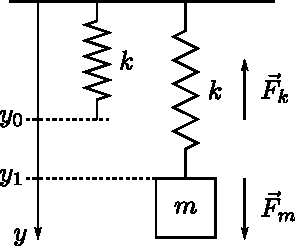
\includegraphics[scale=0.75]{../fig/federpendel-vertikal.pdf}
	\caption{Vertikales Federpendel}
	\label{fig:federpendel-vertikal}
\end{figure}

Der Einfluss der Erdbeschleunigung zeigt sich als \textit{Offset} in
der Bewegungsgleichung
\[ \boxed{x(t) = \underbrace{-\frac{m \cdot g}{k}}_{\text{Offset}} 
	+ A \cdot \cos(\omega \cdot t + \phi)} \]
Die Dynamik des Systems ist jedoch nicht beeinflusst von diesem 
Offset, da die Bewegung die selbe bleibt.
\[ \boxed{\omega = \sqrt{\frac{k}{m}}} \]

\subsection{Energie}
Die Energie eines einfach harmonischen Schwingungssystems verlagert
sich ständig zwischen den beiden Energiespeichern. In den Extremlagen,
also dort wo die Geschwindigkeit maximal und minimal ist, ist die
gesamte Energie jeweils in der Feder bzw. in der Bewegung (kinetische
Energie).
\[ \boxed{E_{pot}(t) = \frac{1}{2} \cdot k \cdot x(t)^2} \]
\[ \boxed{E_{kin}(t) = \frac{1}{2} \cdot m \cdot v(t)^2} \]
Möchte man die Gesamtenergie des Systems so kann man dies für eine
der Extremlagen mittels einer der obigen Formeln berechnen. Für eine
beliebige Lage muss hierfür eine Kombination aus beiden Energien
berechnet werden.
\[ \boxed{E_{tot} = \frac{1}{2} \cdot k \cdot A^2 
= \frac{1}{2} \cdot m \cdot \omega^2 \cdot A^2 
= \frac{1}{2} \cdot m \cdot (v_{max})^2} \]
